% \part{Appendix}\label{part:appendices}
\chapter{An atom temperature optimization routine}\label{ch:tempopt}

To-date, our atoms in the FORT are typically around 100 $\mu \mathrm{K}$, as found a with release-recapture measurement\cite{Tuchendler2008}. Lowering the temperature, for example through adding a dedicated PGC phase or tuning the parameters used for atom readout, has proven largely ineffective. In this appendix, we propose a method which may be suitable given the architectural limitations and capabilitiies of our experimental platform.

Having a sufficiently low atom temperature is important for a number reasons, including for enhancing the survival probability of the atom during sequences which excite the atom, such as optical pumping. Typically, some amount of polarization gradient cooling is acheived not only in the MOT but also during the atom readout, helping to get sub-Doppler temperatures in the FORT. However, imbalanced cooling beams and a non-zero magnetic field at the atom can severely limit the effectiveness of this cooling\cite{chin2017polarization}.

In a more typical cold atom apparatus, the MOT beams are delivered to the vacuum chamber in free space, which makes measuring and setting their powers to be balanced straightforward. Then, the magnetic field can be zeroed, for example, by doing microwave spectroscopy of the hyperfine ground states and adjusting the magnetic shim fields until the different hyperfine transitions become degenerate\cite{Young2022thesis}.

\begin{figure}[!ht]
    \centering
    \includegraphics[width=0.45\textwidth]{Images/beam_balance_and_shims_optimization.pdf}
    \caption{An experiment to optimize the MOT beams and readout shims simultaneously to achieve the lowest atom temperature. Single atoms are loaded then detected with the first readout (RO), then values chosen by an optimization routine are used to set the MOT beam powers and shim coils (green dashes) before an intermediate test "RO". The FORT is turned off for short enough time that some but not all atoms will escape, depending on their temperature distribution. The RO parameters are set back to their defaults (pink dashes) before a final readout. The MOT beams are turned on at the end of the sequence using the test values (blue dashes), and the MOT beam photodetector values are recorded.}
    \label{fig:beam_and_shims_optimization}
\end{figure}

For our fiber-coupled apparatus, where our MOT beam powers can not be directly measured, a single atom experiment can be conducted to simultaneously optimize the balance of the cooling beam intensities at the location of the trapped atom as well as zero the magnetic field. The optimization routine is shown in Fig. \ref{fig:beam_and_shims_optimization}. The experiment is a standard two-readout atom loading routine, but with a "test readout" in the middle followed by a FORT drop. Atoms are either heated or cooled by the intermediate readout which uses parameters chosen by an optimization routine to set the MOT beam powers (by adjusting the RF to the fiber AOMs) and the shim coil values. By maximizing the fraction of atoms which survive the FORT drop, we find parameters that improve the atom temperature. If the parameter space is allowed to be sufficiently large, a global optimization routine (e.g. Bayesian optimization implemented in M-LOOP) should be able to find the point where the MOT beams are balanced and the magnetic field at the atoms is zero.

After running the optimization routine described above, the set points for the beam powers should be set using the best photodetector values. Single atom loading can be found again by scanning the MOT coils, and the readout shims should be optimal using the shim values found in the optimization routine.

To aid the author's successors, here is some ARTIQ python pseudocode for the described optimization routine. The following experiment function would be run with the GeneralVariableOptimizer experiment to optimize the variables $\mathrm{test} \_ \mathrm{amplitude}1$, etc.,  and $\mathrm{AZ} \_ \mathrm{bottom} \_ volts$, etc., shown in the code below. The i2V values corresponding to the best fiber AOM RF amplitudes should then be set as the new set points, and a MOT and single atom loading can be found with the new beam powers by scanning the MOT coils.

\definecolor{codegreen}{rgb}{0,0.6,0}
\definecolor{codegray}{rgb}{0.5,0.5,0.5}
\definecolor{codepurple}{rgb}{0.58,0,0.82}
\definecolor{backcolour}{rgb}{0.95,0.95,0.92}

\lstdefinestyle{mystyle}{
    backgroundcolor=\color{backcolour},   
    commentstyle=\color{codegreen},
    keywordstyle=\color{magenta},
    numberstyle=\tiny\color{codegray},
    stringstyle=\color{codepurple},
    basicstyle=\ttfamily\footnotesize,
    breakatwhitespace=false,         
    breaklines=true,                 
    captionpos=b,                    
    keepspaces=true,                 
    numbers=left,                    
    numbersep=5pt,                  
    showspaces=false,                
    showstringspaces=false,
    showtabs=false,                  
    tabsize=2
}

\lstset{style=mystyle}

\begin{lstlisting}[language=Python
]

def atom_temp_optimization_experiment(self):
    """
    an experiment which can be used to find optimal MOT beam and coil values using an atom in the FORT
    """

    self.set_dataset('i2v_1',[0.0], archive=True)
    self.set_dataset('i2v_2',[0.0], archive=True)
    self.set_dataset('i2v_3',[0.0], archive=True)
    self.set_dataset('i2v_4',[0.0], archive=True)
    self.set_dataset('i2v_5',[0.0], archive=True)
    self.set_dataset('i2v_6',[0.0], archive=True)


    for measurement in range(self.n_measurements):
        self.laser_stabilizer.run()
        load_MOT_and_FORT(self)

        self.zotino.write(self.coil_channels, 
                          [self.AZ_bottom_volts_RO,self.AZ_top_volts_RO,self.AX_volts_RO,self.AY_volts_RO])

        first_shot(self)

        # set the optimization variables:
        self.zotino.write(self.coil_channels, 
                          [self.AZ_bottom_volts_test,self.AZ_top_volts_test,self.AX_volts_test,self.AY_volts_test])

        self.dds_AOM_A1.set(frequency=self.freq_AOM_A1, amplitude=self.test_amplitude1)
        self.dds_AOM_A2.set(frequency=self.freq_AOM_A2, amplitude=self.test_amplitude2)
        self.dds_AOM_A3.set(frequency=self.freq_AOM_A3, amplitude=self.test_amplitude3)
        self.dds_AOM_A4.set(frequency=self.freq_AOM_A4, amplitude=self.test_amplitude4)
        self.dds_AOM_A5.set(frequency=self.freq_AOM_A5, amplitude=self.test_amplitude5)
        self.dds_AOM_A6.set(frequency=self.freq_AOM_A6, amplitude=self.test_amplitude6)

        delay(1*ms)

        # the test cooling phase
        self.dds_cooling.sw.pulse(self.t_recooling)

        self.dds_FORT.sw.off()
        delay(self.t_FORT_drop)
        self.dds_FORT.sw.on()

        # set the usual readout settings:
        self.zotino.write(self.coil_channels, 
                          [self.AZ_bottom_volts_RO,self.AZ_top_volts_RO,self.AX_volts_RO,self.AY_volts_RO])

        # use the fiber AOM amplitudes from the most recent feedback run
        self.dds_AOM_A1.set(frequency=self.freq_AOM_A1, amplitude=self.stabilizer_AOM_A1.amplitude) 
        self.dds_AOM_A2.set(frequency=self.freq_AOM_A2, amplitude=self.stabilizer_AOM_A2.amplitude)
        self.dds_AOM_A3.set(frequency=self.freq_AOM_A3, amplitude=self.stabilizer_AOM_A3.amplitude)
        self.dds_AOM_A4.set(frequency=self.freq_AOM_A4, amplitude=self.stabilizer_AOM_A4.amplitude)
        self.dds_AOM_A5.set(frequency=self.freq_AOM_A5, amplitude=self.stabilizer_AOM_A5.amplitude)
        self.dds_AOM_A6.set(frequency=self.freq_AOM_A6, amplitude=self.stabilizer_AOM_A6.amplitude)

        second_shot(self)

        # check what values the i2Vs measure at the optimizer settings for the AOM amplitudes-- we want to use these values as the new MOT beam set points once we find the best iteration from the optimization run.

        buffer = [0.0]*8
        self.sampler0.measure(buffer) # should probably average this
        i2v_1 = buffer[self.stabilizer_AOM_A1.buffer_index]
        i2v_2 = buffer[self.stabilizer_AOM_A2.buffer_index]
        i2v_3 = buffer[self.stabilizer_AOM_A3.buffer_index]
        i2v_4 = buffer[self.stabilizer_AOM_A4.buffer_index]
        i2v_5 = buffer[self.stabilizer_AOM_A5.buffer_index]
        i2v_6 = buffer[self.stabilizer_AOM_A6.buffer_index]

        self.append_to_dataset('i2v_1',i2v_1)
        self.append_to_dataset('i2v_2',i2v_2)
        self.append_to_dataset('i2v_3',i2v_3)
        self.append_to_dataset('i2v_4',i2v_4)
        self.append_to_dataset('i2v_5',i2v_5)
        self.append_to_dataset('i2v_6',i2v_6)

        end_measurement(self)

\end{lstlisting}




